\documentclass[11pt,a4paper]{report}
\usepackage{ifpdf}
\usepackage[utf8]{inputenc}
\usepackage[francais]{babel}
\usepackage[french]{varioref} 
\usepackage[pdftex]{graphicx}
\usepackage{listings}
\usepackage{color}
\usepackage{amssymb}
\usepackage{amsmath}

%\usepackage{floatflt}
\usepackage{lscape} %afficher une partie en paysage


%%% Pour du code source %%%%
 \definecolor{colKeys}{rgb}{0.5,0,0.33} 
 \definecolor{colIdentifier}{rgb}{0.16,0,1} 
 \definecolor{colComments}{rgb}{0.25,0.5,0.37} 
 \definecolor{colString}{rgb}{0.6,0.1,0.1} 
 \definecolor{shadow}{rgb}{0.5,0.5,0.5} 
 
 \lstset{ 
 basicstyle=\ttfamily\small,
 identifierstyle=\color{colIdentifier},
 keywordstyle=\color{colKeys},
 stringstyle=\color{colString},
 commentstyle=\color{colComments}
 }
 \lstset{language=python}



\begin{document}

%\tableofcontents
\thispagestyle{empty}
\begin{center}
\begin{tabular}{lr}
\begin{minipage}[l]{0.4\textwidth}
\begin{flushleft}

\includegraphics[scale=0.2]{logo.png}
\end{flushleft}
\end{minipage}
&
\begin{minipage}[r]{0.4\textwidth}
\begin{flushright}
\begin{tabular}{l}
Van De Walle Bernard  (A)\\
Francois Thibault (B) \\
Van Der Essen Frédéric (C)
\end{tabular}
\end{flushright}
\end{minipage}
\end{tabular}
\end{center}

\vspace{6.5cm}

\begin{center}
\textsc{INGI2132: Langages et traducteurs}
\end{center}

\bigskip

\begin{center}
{\Huge Rapport Final}
\end{center}

\vspace{7.5cm}
\begin{center}
		\textbf{Prof.} B. Le Charlier\\
\end{center}

\vspace{1.5cm}

\newpage

\begin{figure}[h!]
\begin{center}
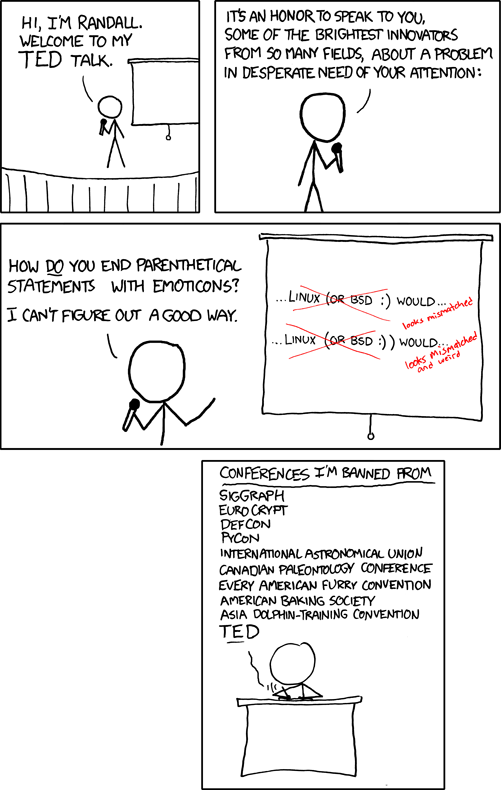
\includegraphics[scale=0.65]{xkcd.png}
\end{center}
\end{figure}
It is now possible with the HAPPY-) programming language !
\newpage


%3
\chapter{Présentation de Happy:-)}
\section{Introduction}
La langage happy, appelé ainsi parce qu'il est très permissif au niveau des caractères permit dans les identifiants comporte de nombreuses autres particularités. Tout d'abord, le langage ressemble très fort au LISP où tout est atom ou liste.
Mais contrairement au LISP, notre langage est impératif et orienté objet. Un programme est une liste de méthode, une méthode est une liste dont le premier élément est le mot réservé fun le second une list d'argument et le dernier une liste de commande. Même principe pour le while et le if. Dans ce langage tout est fonction, dans le sens que toute instruction renvoie une valeur, y compris les if et le while qui renvoient 0, une fonction qui n'a pas d'instruction return renvoie null, le write renvoie la valeur qu'elle vient d'imprimer etc...



Les conditions aurait aussi renvoyé une valeur si le langage SLIP dans lequel notre langage est traduit le permettait. 

\section{Grammaire de départ}
Cette grammaire est la grammaire exhaustive du langage si on rajoute que les id peuvent être formé de tout les caractères UTF-16 sauf des caractères réservés et qu'ils ne doivent pas être égale à un mot réservé.

\begin{verbatim}
<Program> ::= ( <Prog_list> )
<Prog_list> ::=  <Meth_or_fun> | <Prog_list> <Meth_or_fun>	
<Meth_or_fun> ::=  <Method> | <Function>

<Function> := ( fun ( <Arglist> ) <Instr_list> ) 
<Arglist> ::=  id | id <Arglist>
<Method> ::= ( <Method_int> ( <Arglist> ) <Instr_list> )
 
<Instr_list> ::=  <Instr> | ( <Instr_list_np> ) 
<Instr_list_np> ::=  <Instr> | <Instr> <Instr_list_np>
<Instr> ::=  <Conditional> | <While_block> | <Call> | ( return <Expr> ) 

<Conditional> ::= ( if <Cond> <instr_list> <instr_list>  )  
<Conditional> ::= ( if <Cond> <instr_list> )
<While_block> ::= ( while  <Cond> <Instr_list>  ) 
<call> ::=  <User_call> | <Method_call> | <Builtin_call> 
<Builtin_call> ::=  <Assignment> | <Read_call> | <Write_call> | <Arithmetic_call>
<Assignment> ::= ( set id <Expr> ) 
<Assignment> ::= ( set <Id_int> <Expr> ) | ( set <This_int> <Expr> )
<Read_call>  ::= ( read )
<Write_call> ::= ( write <Expr> )
<Arithmetic_call> ::=  <Binary> | <Unary>
<Binary> ::= ( <Bin_id> <Expr> <Expr>  )
<Unary>  ::= ( <Un_id> <Expr>  )
<User_call>  ::= ( id  <Expr_list_np> ) | ( id ) 
<Expr_list_np> ::=  <Expr> | <Expr> <Expr_list_np>
<Method_call>  ::= ( <Id_id> <Expr_list_np>  ) |  ( <Id_id> )   
<Method_call>  ::= ( <Super_id>  <Expr_list_np>  ) | ( <Super_id>  )
<Method_call>  ::= ( <This_id>  <Expr_list_np>  ) | ( <This_id> )
<Expr> ::= number | null | true | false | this | id 
<Expr> ::= <Id_int> | <This_int> | <Instr>
<Cond> ::= <Rel> | ( <Log_bin_op> <Cond> <Cond> )
<Cond> ::= ( <Log_un_op> <Cond> <Cond> )
<Rel>  ::= ( <Rel_op> <Expr> <Expr> ) 
<Rel_op> ::= <= | >= | > |  < | =
<Log_bin_op> ::= and | or
<Log_un_op> ::= !
<Bin_id> ::= + | - | * | / | %
<Un_id> ::= neg
<Id_int> ::= id . number
<This_int> ::= this . number
<Super_id> ::= super . id
<This_id> := this . id 
<Id_id> ::= id . id
<Method_int> ::= method . number
\end{verbatim}
Cette grammaire n'est pas wp, mais elle exprime très bien ce qui est syntaxiquement correcte dans ce que nous avons réellement implémenté. 

Voici quelque bout de code permis par cette grammaire :

\begin{verbatim}
[Le while s'écrit comme ceci while (la condition) (les instruction a répèter)
  ici la condition est 3 * i <= 9
On remarque aussi que sur ce bout de code on peut écrire 
la valeur de retour de set qui sera ici i_initial + 1 ou i_final ]
(while (<= (* 3  i) 9) (write (set i (+ i 1)))) 
  
[Condition ici si i != 9 ]
[Ensuite si vrai on exécute la première list d'instruction sinon la seconde]
(if (! (= i 9)) (return true) (return false))
[Ceci est équivalent à sauf que dans le cas deux on voit clairement les listes d'instructions]
(if (! (= i 9)) ((return true)) ((return false)))

(fun (++ i) (return (+ i 1)))

(set i (++ i))

(set a (new 2))
\end{verbatim}

\section{Exemple de programme complet}
Le premier programme imprime juste l'entier lu à la console.

\begin{verbatim}
(
  (fun (main) 
    (write (read))
  )
)
\end{verbatim}

Le programme suivant fait la somme de 1 à n pour 10 n
\begin{verbatim}
(
  [Programme fait la somme de 1 à n pour n qui va de 0 à 10]
  (fun (main) (
    (set i 0)
    (while (<= i 10)
    (
      (write (sum i))
      (set i (+ i 1))
    ))
  ))


  (fun (sum n) (
    (if (= n 0)
      (return 0)
    )
    (return (+ n (sum (- n 1))))
  ))
)

\end{verbatim}



Le dernier programme fait la somme des éléments d'une pile et utilise la POO
\begin{verbatim}
(
  (fun (main) (
    (set s ( >> 4 ( >> 3 (>> 2 (# 1)))))
    (write (s.@))
    (write (s.->))
    (set s (>> 5 s))
    (Print s)
    (write (sum s))
  ))
  [crée une nouvelle pile avec a comme élément au sommet]
  (fun (# a) (
    (set b (new 2))
    (b.@= a)
    (b.->= null)
    (return b)
  ))

  [Push sur la stack]
  [a : l'élément à mettre sur la stack]
  [s : la stack]
  (fun (>> a s) (
    (set n (new 2))
    (n.->= s)
    (n.@= a)
    (return n)
  )) 

  (fun (Print N) (
    (if (! (= N null)) (
      (write (N.@))
      (Print (N.->))
    )
    (write 0)
    )
  ))

  (fun (sum N) (
    (if (! (= N null)) 
      (return (+ (N.@) (sum (N.->))))
      (return 0)
    )
     
  ))
  [Accesseur pour l'élément contenu dans le noeud]
  (method.2 (@) (return this.1))
  ((method.2 (@= a) (set this.1 a))
  [Accesseur pour next]
  (method.2 (->) (return this.2))
  (method.2 (->= a) (set this.2 a))
)
\end{verbatim}




 

%10
\chapter{Mode d'emploi du compilateur}
La version exécutable du compilateur et interpréteur Happy se trouve dans le jar exécutable \textit{happy.jar}.
Il prend 2 arguments obligatoire : la grammaire au format BNF et le programme en langage Happy. On peut rajouter \textit{check} à la fin pour vérifier la grammaire en plus.
Pour faire fonctionner les programmes Happy, il faut passer la grammaire \textit{temp.bnf}. Pour vérifier n'importe quelle grammaire WP, il faut indiquer la grammaire
un fichier programme bidon et enfin check.
exemple : \begin{verbatim}
    java -jar happy.jar temp.bnf programme1.happy 
    java -jar happy.jar temp.bnf programme1.happy check
          \end{verbatim}

L'interpréteur sort les informations suivantes dans cet ordre, si le check de la grammaire est demandé, le résultat des tests et la table de précédence.
Ensuite l'arbre sortit par le parser syntaxique après sa restructuration, ensuite la traduction de l'arbre en SLIP et puis (mais il semble que
les retour à la ligne ne soit pas conforme ce qui donne des résultats étranges à la sortie dans le shell) la représentation en code interne SLIP. Et finalement
la sortie du programme interprèté. 


\section{Les erreurs}
Lorsqu'une erreur arrive dans n'importe quelle partie du compilateur l'erreur est affichée (avec plus ou moins de précision) et il s'arrête ensuite.
\section{Les erreurs du vérificateur}
  

\section{Les erreurs du parser lexical}
  Il ne vérifie que deux choses. A la fin de l'analyse si il n'y a pas le même nombre de paranthèse ouvrantes que fermantes, l'erreur \textit{Unexpected end}.
  Il est aussi capable de vérifier si à tout moment il y a trop de paranthèse fermantes, le messages est dès lors très explicite : \textit{Too much ) }.
\section{Les erreurs de l'analyseur syntaxique}
  L'analyseur syntaxique signale trois erreurs. Lorsque deux termes ne peuvent se retrouver côte à côte, lorsqu'il n'arrive pas à trouver une règle pour réduire.


Et lorsqu'il a lu tout les caractères, si il reste plus d'un élément dans la pile une erreur est aussi renvoyé.
\section{Les erreurs du traducteur}
    Les erreurs que renvoient le traducteur sont d'ordre sémantique. Le programme est valide syntaxiquement mais comme notre grammaire permet beaucoup de chose,
Il faut remettre les choses en places avec le traducteur. Les erreurs sont du type : quelquechose est attendu dans ce type d'expr et là c'est pas le cas. 
exemple : textit{Expected id after a set}


\section{Les erreurs de l'interpréteur}
  L'interpréteur reporte les erreurs d'exécutions telles que la division par 0, l'appel à méthode inconnue etc...
  Les erreurs sont clairement identifié dans le code interne structurée et reporté jusqu'au dessus de la pile d'exécution. Cela permet de retracer l'erreur
sans trop de difficulté. 
Voici un exemple : 
\begin{verbatim}
Error divide by 0
	 in Cexpr a#1 / b#2
	 at Ass A_0#3 := a#1 / b#2
	 at CmdStmt [ lab9 : A_0#3 := a#1 / b#2 ; go to lab8]
	 at divide/-1
	 at Call divide
	 at CmdStmt [ lab2 : A_0#3 := divide(#4, #5) ; go to lab1]
	 at main/-1
\end{verbatim}

\end{document}
